\documentclass[12pt, a4paper]{article}
\usepackage{fontspec}
\setmainfont{Times New Roman}
\usepackage[UTF8]{ctex}
\usepackage{listings}
\usepackage{array}
\usepackage{geometry}
\geometry{a4paper, scale=0.75}
\usepackage{ctex}
\usepackage{amsmath}
\usepackage{epsfig}
\usepackage{graphicx}
\usepackage{epstopdf}
\usepackage{cite}
\usepackage{indentfirst}
\setlength{\parindent}{2em}
\setlength\parskip{.3 \baselineskip}
\usepackage{graphicx}
\usepackage{float}
\usepackage{subfigure}

\begin{document}
	\begin{center}
		\vspace{0.2in}
		\noindent{\fontsize{20pt}{1em}\selectfont\textbf{通信电路\quad 第四周作业}} \\ [12pt]
		\noindent{\fontsize{20pt}{1em}\textbf{Cadence报告}}  \\ [12pt]
		{\fontsize{14pt}{1.2em}\selectfont
			刘开济\\ [10pt]
			2019010973 \\ [10pt]
		}
	\end{center}
    \section{噪声仿真}
    首先考察CS组态放大器如下图:
        \begin{figure}[H]
    	\centering
    	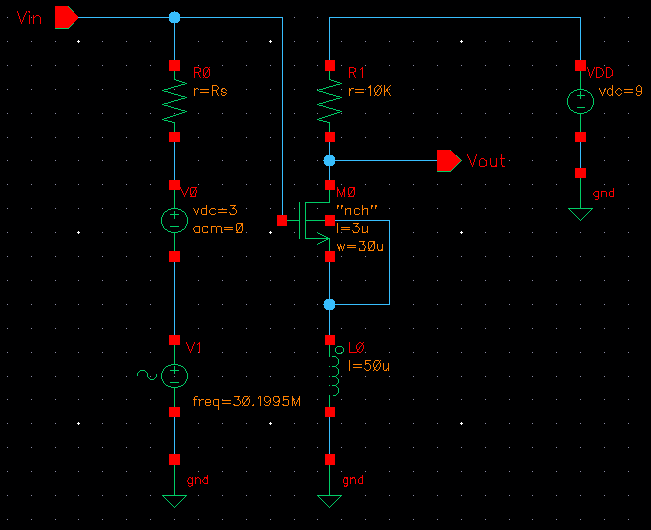
\includegraphics[width = 0.8\textwidth]{CS-noise}
    	\caption{CS Amplifier}
    	\label{Fig2.1}
    \end{figure}\par
    扫描直流工作点如下:
     \begin{figure}[H]
    	\centering
    	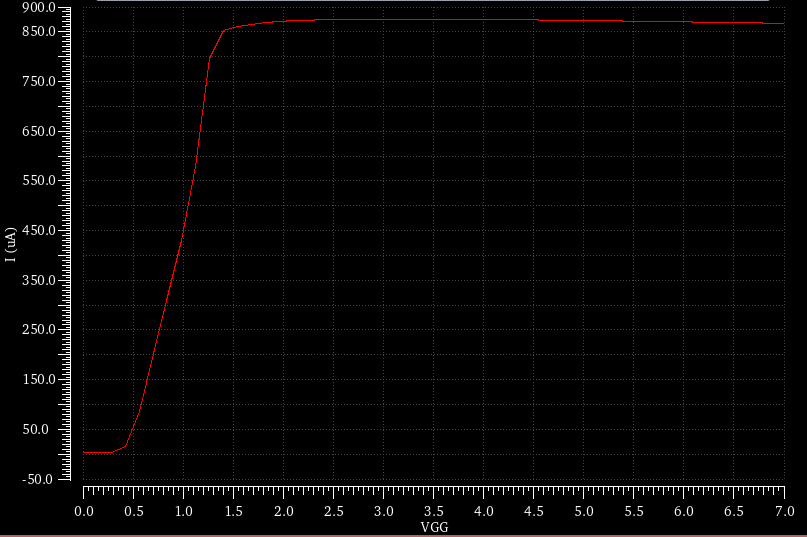
\includegraphics[width = 0.8\textwidth]{CS-noise-DC}
    	\caption{直流工作点}
    \end{figure}\par
    扫描小信号特征如下:
    \begin{figure}[H]
    	\centering
    	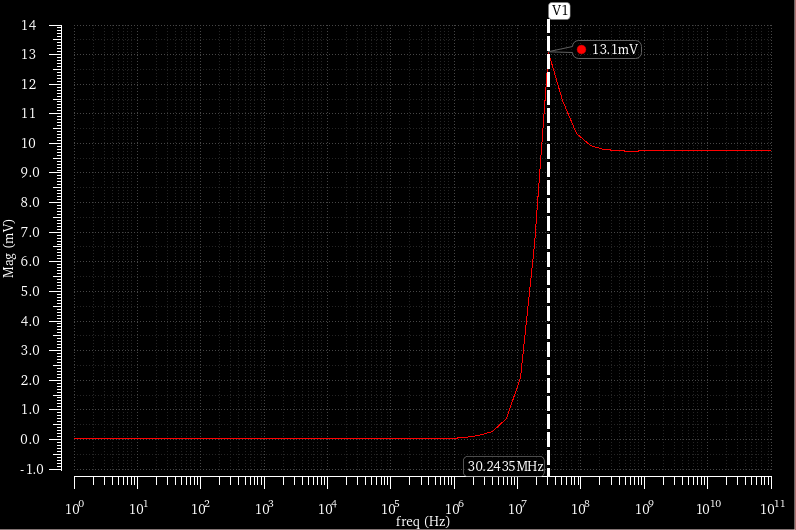
\includegraphics[width = 0.8\textwidth]{CS-noise-AC}
    	\caption{小信号放大}
    \end{figure}\par
    工作频点下的噪声性能如下:
    \begin{figure}[H]
    	\centering
    	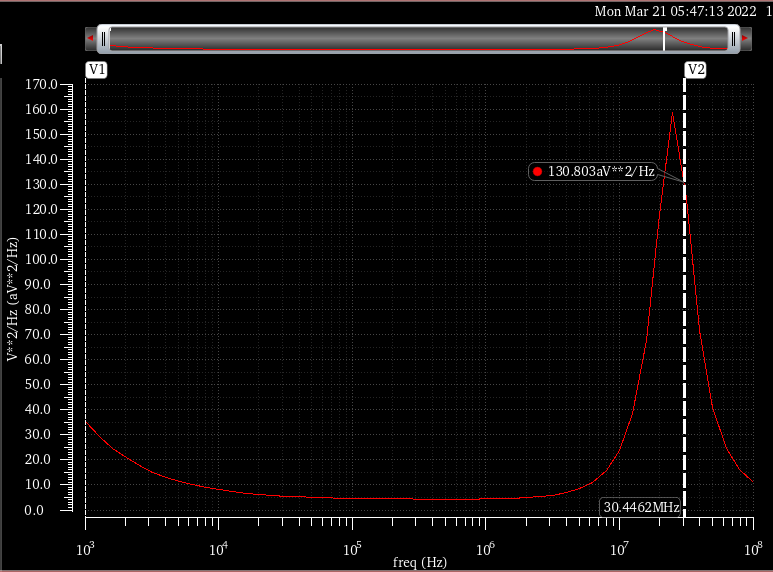
\includegraphics[width = 0.8\textwidth]{CS-noise-noise}
    	\caption{噪声性能}
    \end{figure}\par
    扫描信源内阻$R_s$,有性能如下:
    \begin{figure}[H]
    	\centering
    	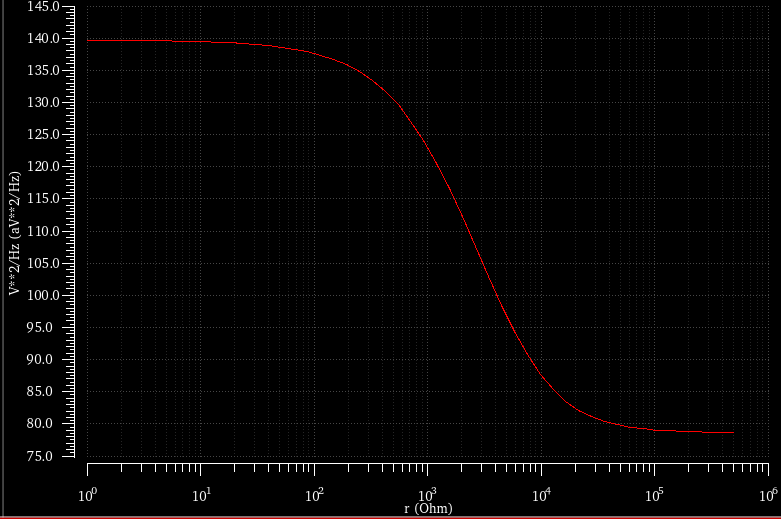
\includegraphics[width = 0.8\textwidth]{CS-noise-Rs}
    	\caption{噪声性能}
    \end{figure}\par
\end{document}